\subsection{Design of Second-Order Low-Pass Filter}

A second-order low-pass filter attenuates frequencies above the cutoff frequency more sharply than a first-order filter, typically providing a slope of $-40$ dB/decade. These filters are commonly used in signal processing to allow low-frequency signals to pass while reducing high-frequency noise or interference.

In this design, we use the Sallen-Key topology which is widely implemented due to its simplicity and effectiveness using op-amps. The standard Sallen-Key configuration is shown below:

\begin{figure}[H]
    \centering
    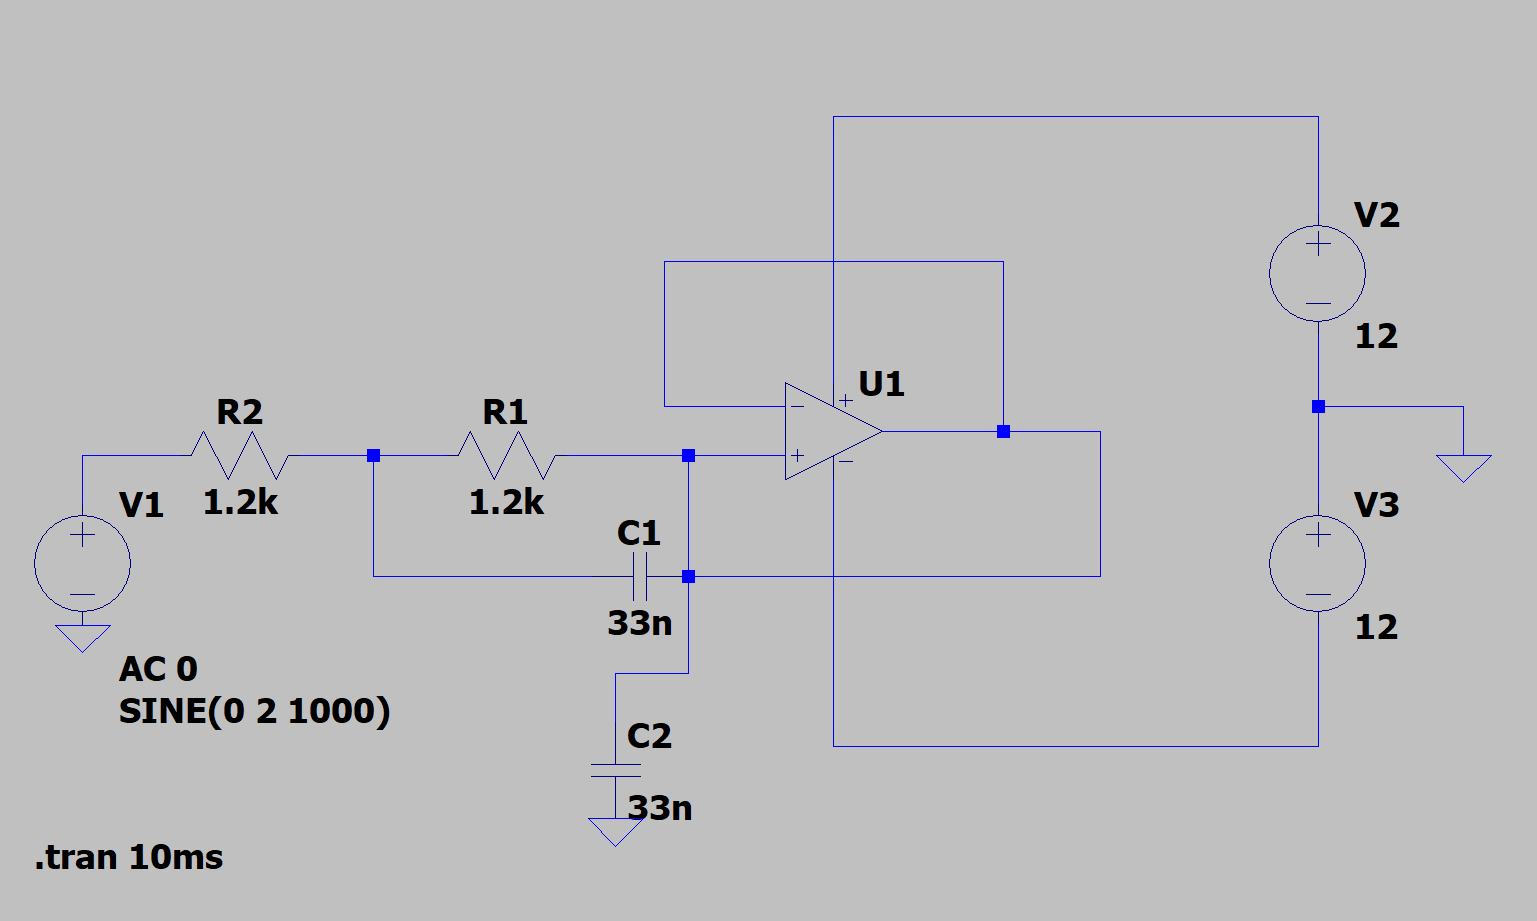
\includegraphics[width=0.9\linewidth]{sec/low-pass/helloworld.png}
    \caption{Sallen-Key Second-Order Low-Pass Filter}
    \label{fig:sallen-key}
\end{figure}

\begin{figure}[H]
    \centering
    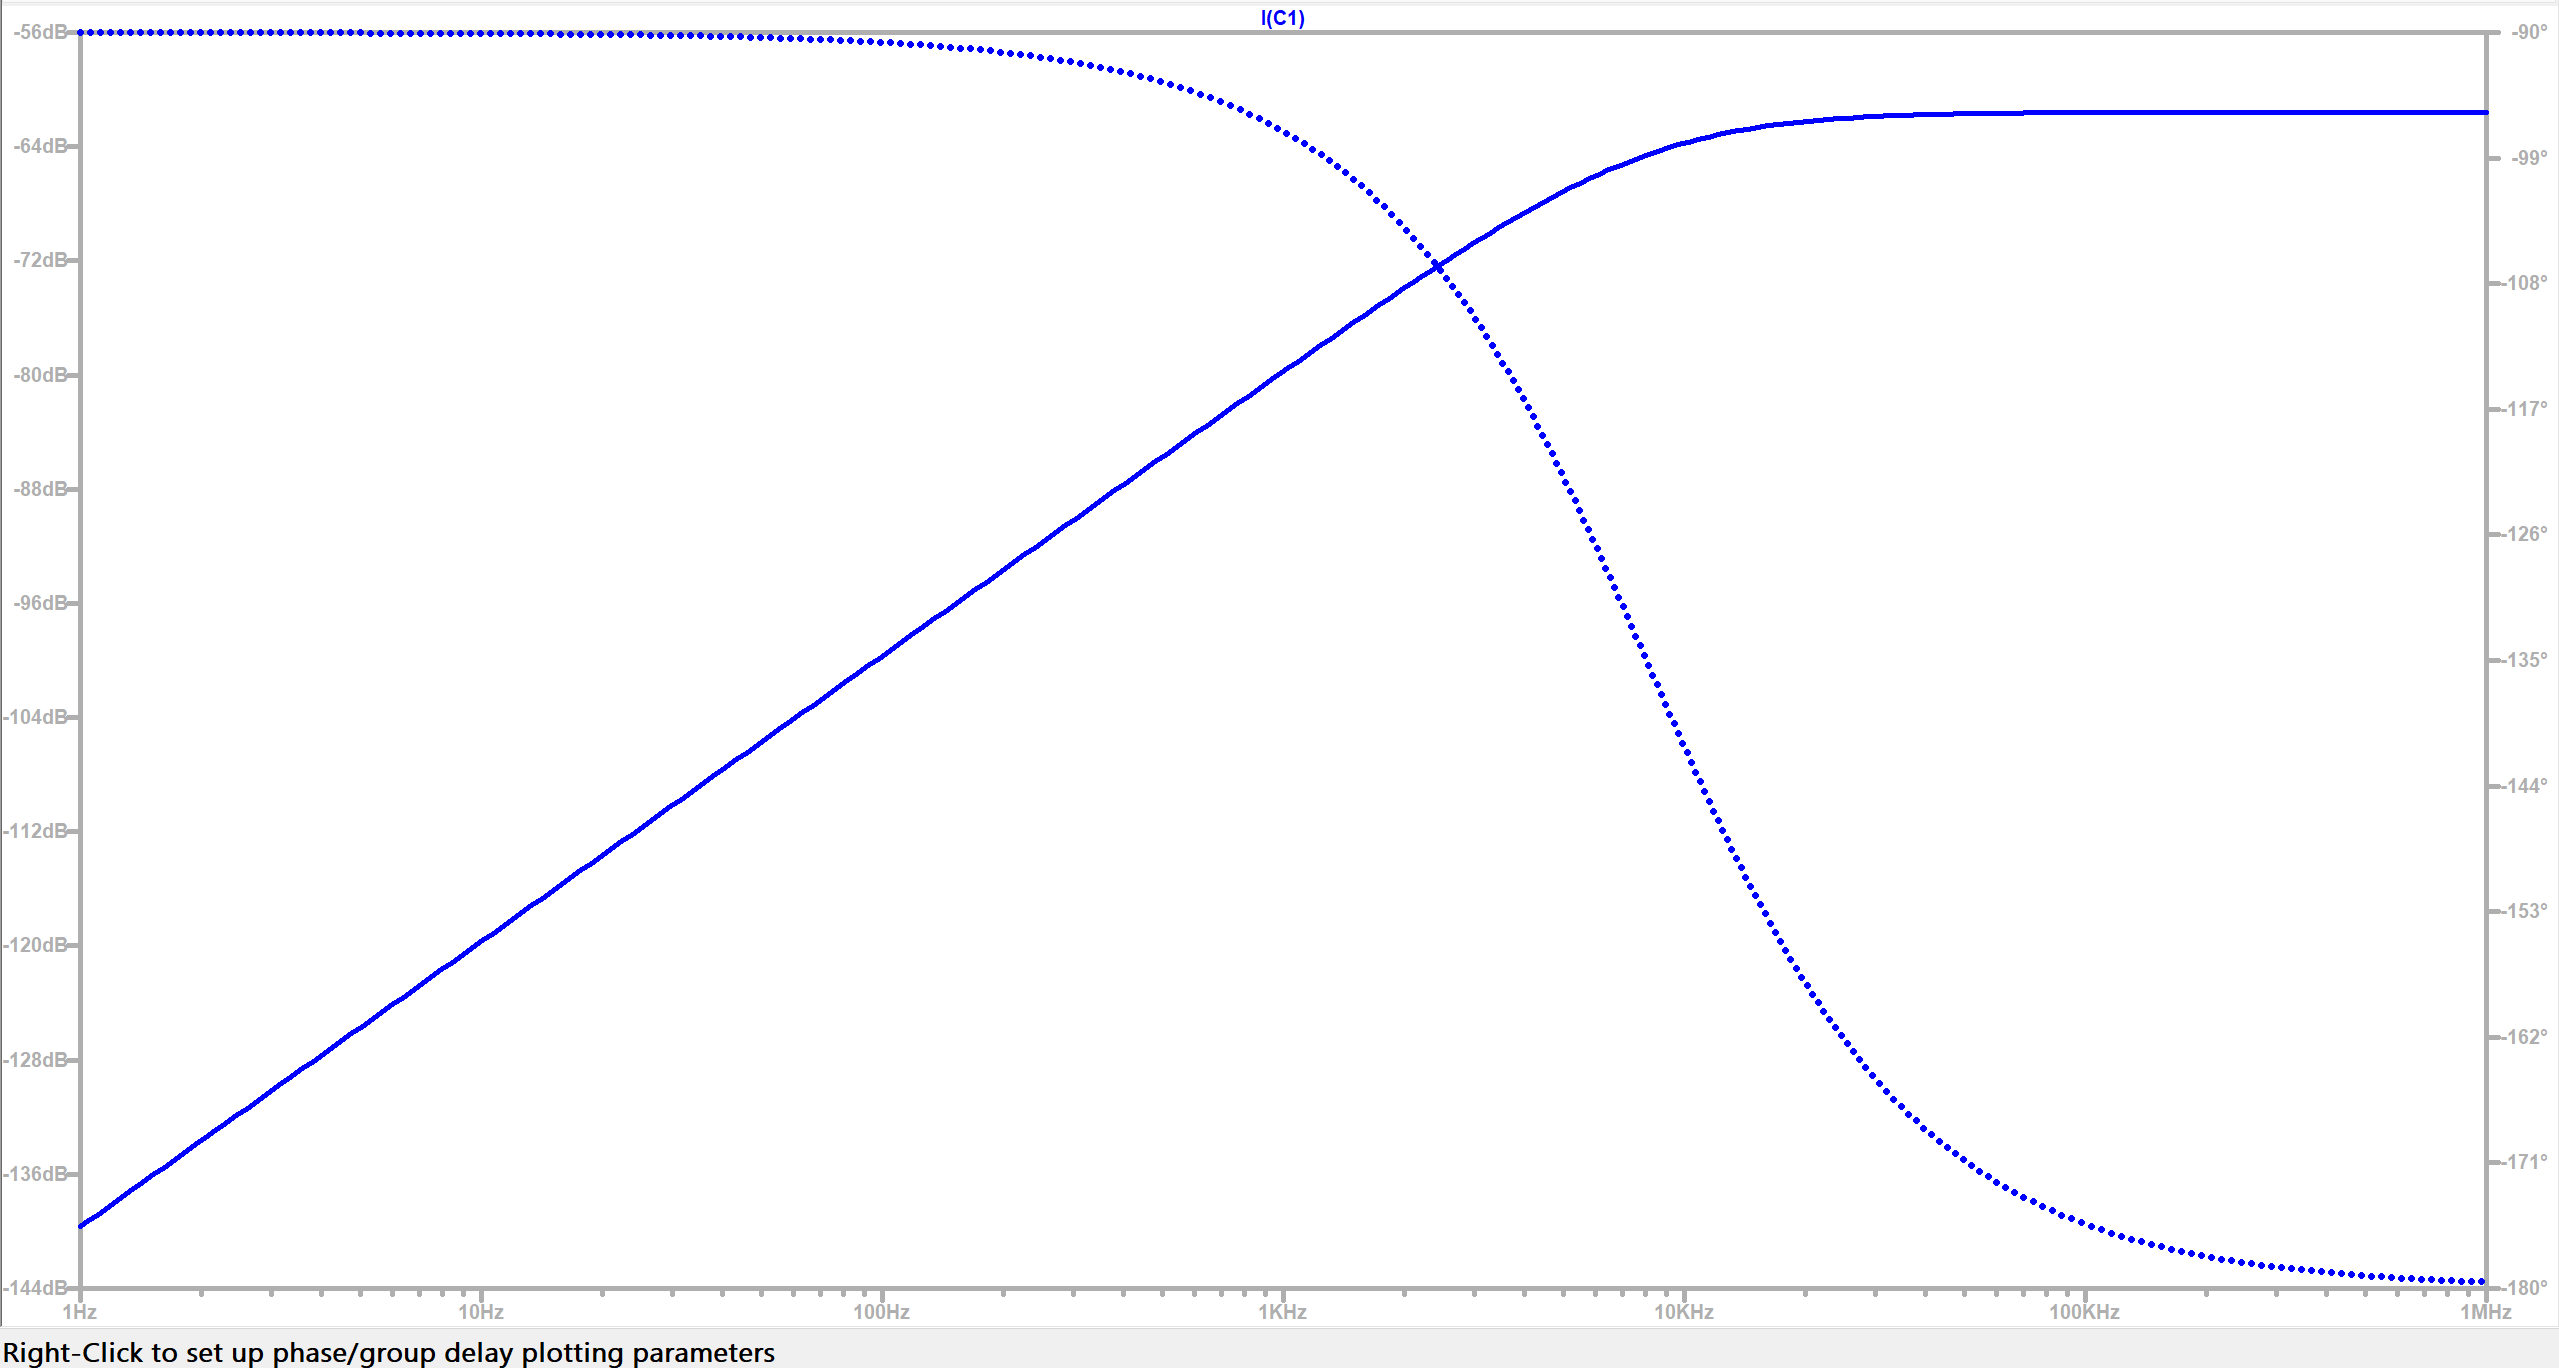
\includegraphics[width=0.95\linewidth]{sec/low-pass/image.png}
    \caption{Bode Plot of Low Pass Filter}
    \label{fig:enter-label}
\end{figure}

The transfer function of a Sallen-Key low-pass filter is given by:

\[
H(s) = \frac{1}{s^2 R_1 R_2 C_1 C_2 + s(R_1 C_1 + R_1 C_2 + R_2 C_2) + 1}
\]

Assuming $R_1 = R_2 = R$ and $C_1 = C_2 = C$ for simplicity, the transfer function becomes:

\[
H(s) = \frac{1}{s^2 R^2 C^2 + 3sRC + 1}
\]

The cutoff frequency $f_c$ of the filter is given by:

\[
f_c = \frac{1}{2\pi RC}
\]

We are designing a low-pass filter with a cutoff frequency of $f_c = 100~\text{kHz}$. Choosing $C = 1~\text{nF}$, we can compute $R$ as:

\[
R = \frac{1}{2\pi f_c C} = \frac{1}{2\pi \cdot 10^5 \cdot 10^{-9}} \approx 1.59~\text{k}\Omega
\]

Selecting a standard resistor value, we choose $R = 1.6~\text{k}\Omega$.

\subsubsection*{Simulation and Response}

When this circuit was simulated using the values:
\[
R_1 = R_2 = 1.6~\text{k}\Omega, \quad C_1 = C_2 = 100~\text{nF}
\]

the output showed a sharp cutoff near $1000~\text{kHz}$ as expected. The gain at low frequencies remained nearly constant (unity gain), and the attenuation slope beyond the cutoff was approximately $-40$ dB/decade, confirming the second-order behavior.

\begin{figure}[H]
    \centering
    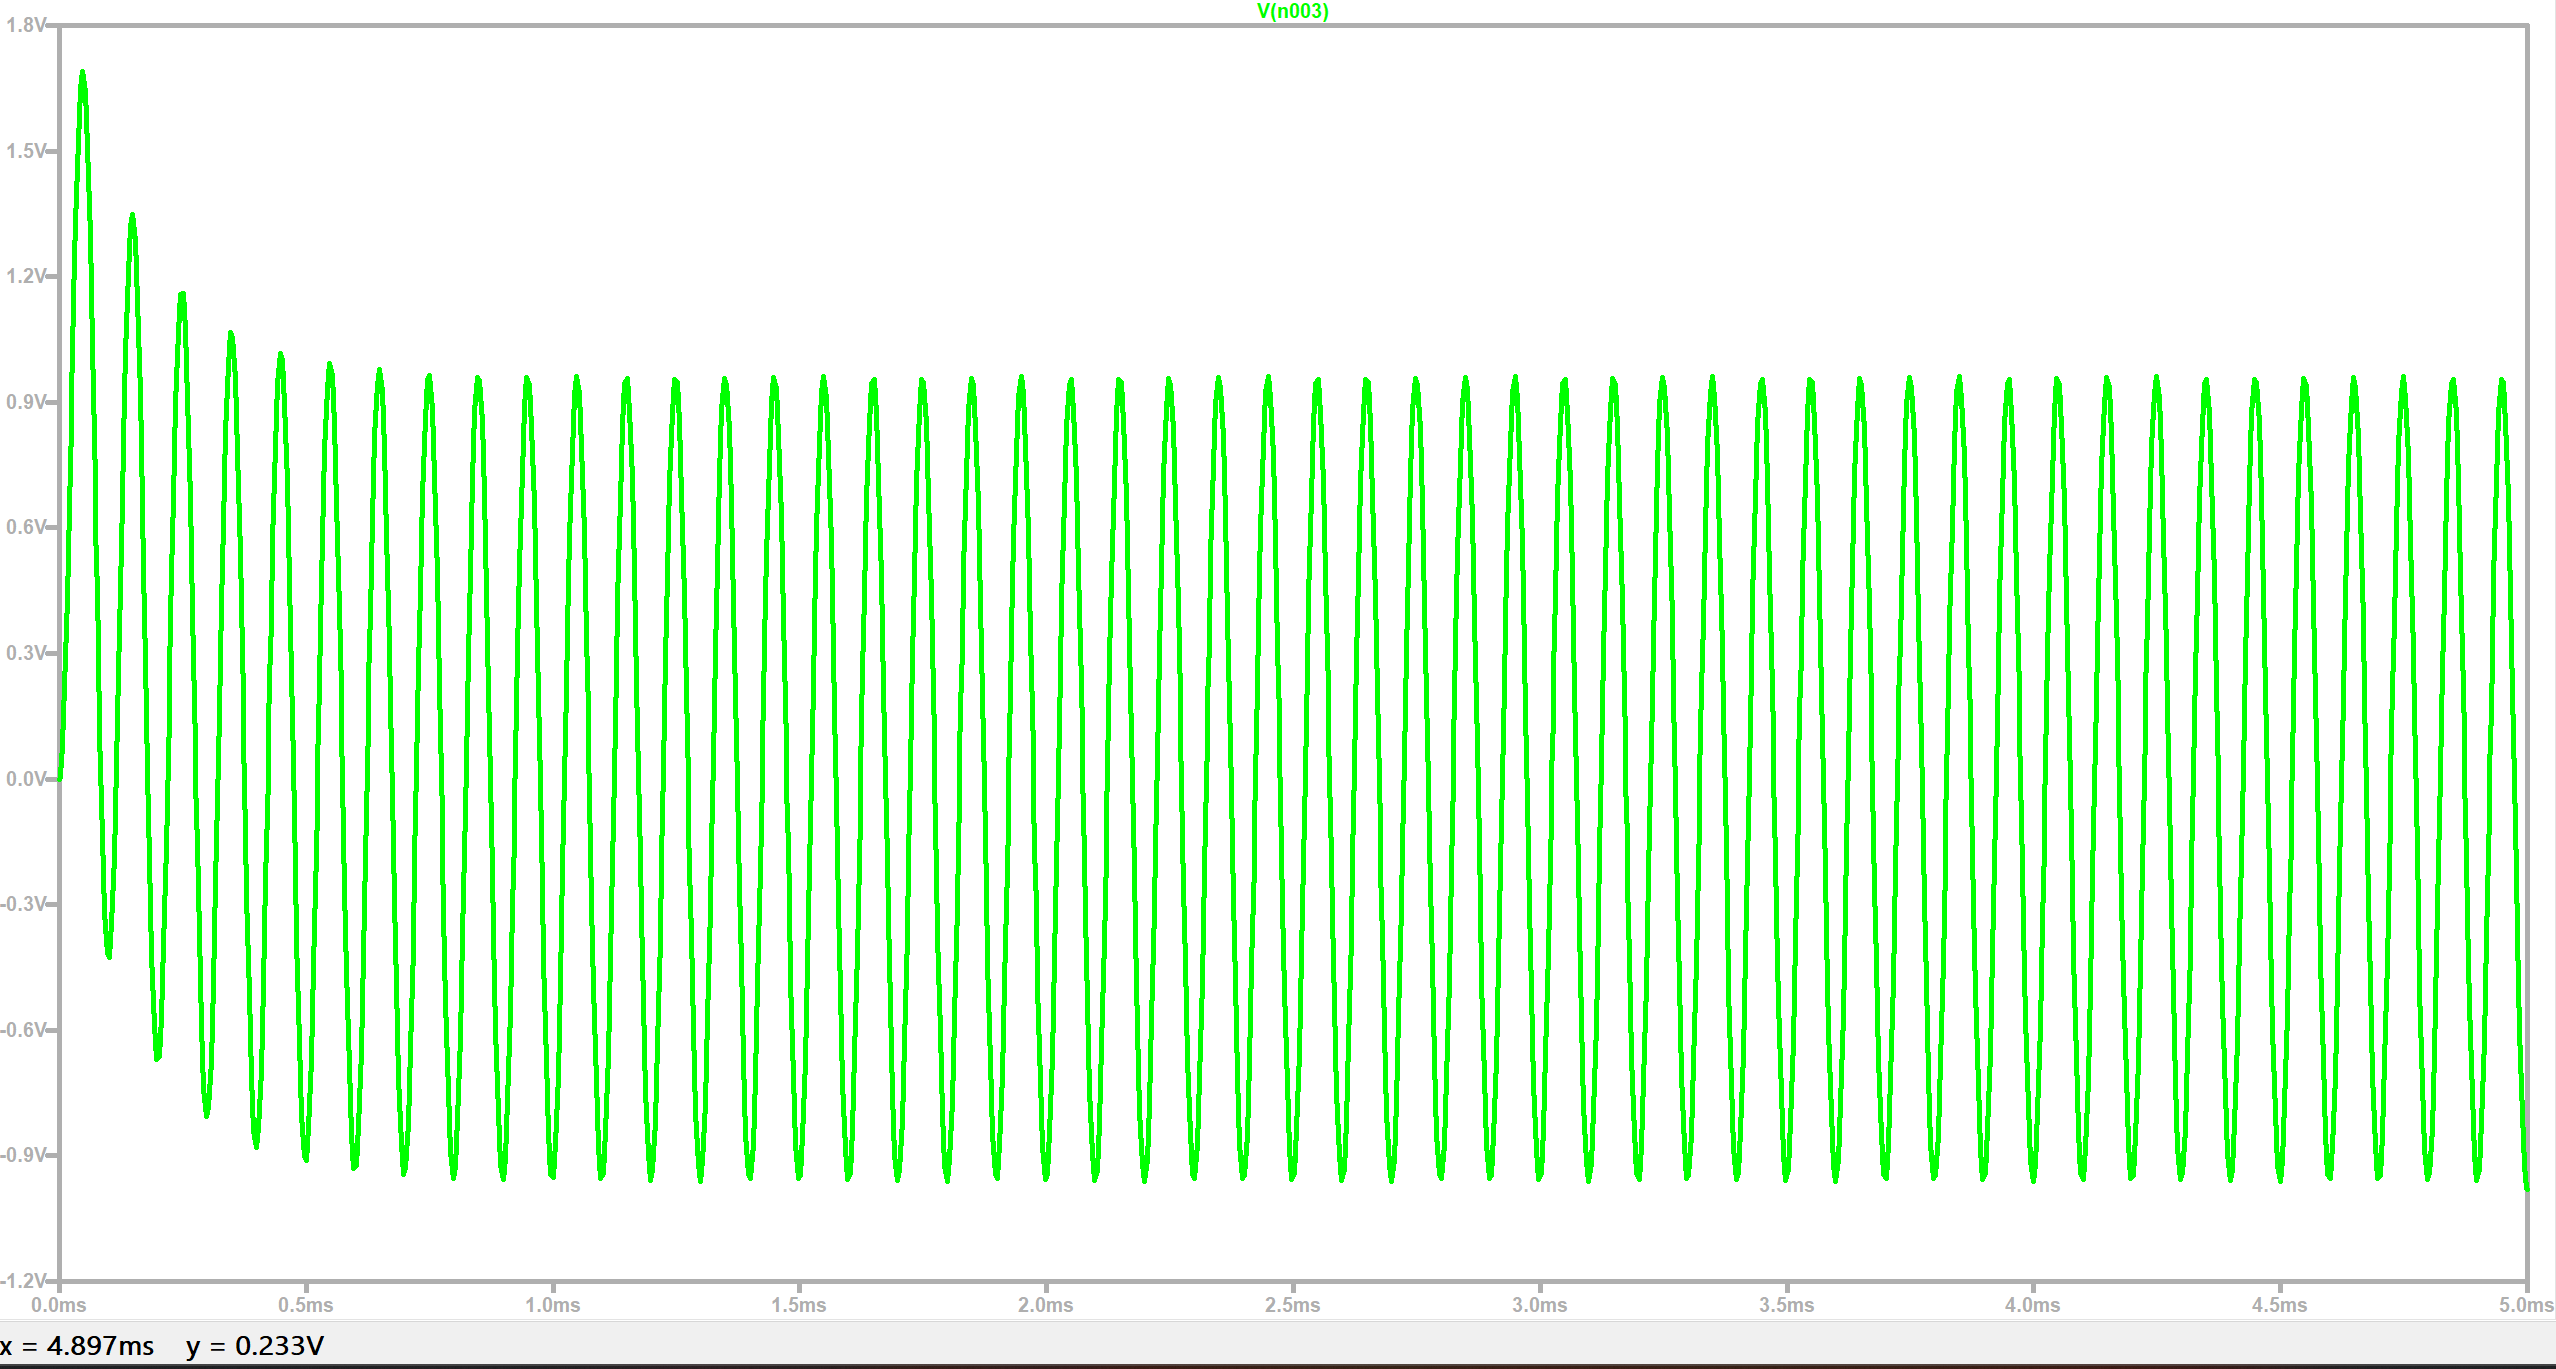
\includegraphics[width=1\linewidth]{sec/low-pass/asd.png}
    \caption{Frequency response of the Second-Order Low-Pass Filter}
    \label{fig:low-pass-response}
\end{figure}

This low-pass filter can be used in signal conditioning, especially to remove high-frequency noise from the oscillator or as a component in larger analog signal processing systems.


\subsection*{Importance of Second-Order Low-Pass Filter in a Quadrature Down-Converter}

In a \textit{quadrature down-converter}, the incoming RF signal is mixed with two local oscillator (LO) signals that are $90^\circ$ out of phase, producing the \textbf{in-phase (I)} and \textbf{quadrature (Q)} baseband components. This mixing operation generates both sum and difference frequency components.

\begin{itemize}
    \item The desired \textbf{baseband signal} appears near 0 Hz (difference frequency: RF$-$LO).
    \item Unwanted \textbf{high-frequency components}, such as the sum frequency (RF$+$LO), also appear in the mixer output.
\end{itemize}

To isolate the baseband I/Q signals, a \textbf{low-pass filter (LPF)} is applied. Specifically, a \textbf{second-order low-pass filter} is preferred due to its sharper roll-off and better attenuation of out-of-band signals compared to first-order filters.

\paragraph{Key Benefits of Using a Second-Order LPF:}
\begin{enumerate}
    \item \textbf{Sharper Cutoff:} Second-order filters have a roll-off rate of $-40~\text{dB/decade}$, providing more effective suppression of high-frequency mixer products.
    
    \item \textbf{Improved Selectivity:} It better isolates the desired baseband signal by reducing adjacent channel interference.
    
    \item \textbf{Anti-Aliasing Protection:} When followed by analog-to-digital conversion (ADC), the LPF prevents aliasing by attenuating frequencies above the Nyquist limit.
    
    \item \textbf{Noise Reduction:} Suppresses out-of-band noise, improving the signal-to-noise ratio (SNR) of the baseband signal.
    
    \item \textbf{Defines Bandwidth:} The filter determines the usable signal bandwidth and thus helps shape the system's frequency response.
\end{enumerate}
